\chapter{16 Tales 1}

The first of the four 16 Tales games published and released by The Lightspan Partnership for the PlayStation 1. Each game consists of four 15-minute video programs various cultures' stories and lore.

16 Tales 1 features a series of four Native American stories, including:
\begin{itemize}
    \item The Angry Moon %\href{https://www.goodreads.com/book/show/24890.The_Angry_Moon?from_search=true & from_srp=true              & qid=GFQW4v18PS   & rank=1}{Link to equivalent book on Goodreads} \\
    \item Coyote and Cottontain \& Coyote and the Beaver People
    \item The Dancing Stars \& The Friendly Wolf
    \item The Fire Bringer \& How Saynday Borought the Buffalo to the Indians
\end{itemize}

Music used throughout:
- Sun Valley by David Snell

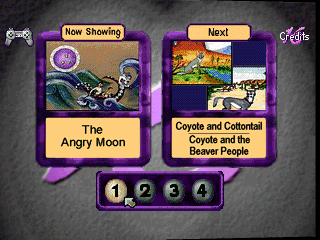
\includegraphics[width=\textwidth]{"./16Tales1Screenshot.png"}

\begin{table}[h]
    \centering
    \begin{small}

        \begin{tabular}{|p{1.5cm}|p{7cm}|p{7cm}|}
            \hline
            \textbf{Story Title} & \textbf{Short Description} & \textbf{Credits} \\
            \hline
            The Angry Moon
                                 &
            A story based on a Native American legend from the Tlingit people in Alaska.
            Adapted from a legend of the Tlingit Indians of Alaska, this book follows Lupan and Lapowinsa and their adventure to the sky country.
            Lupowinsa laughs at the moon and is taken as prisoner by the Moon as punishment.
            Fearing his friends welfare, Lupan makes a ladder of arrows up to sky country.
            With the help of old grandmother, Lupan is given four gifts to help defeat the Moon and save his friend.
                                 &
            Told by: Ginny Taylor
            Producer: K. Hamamura Nelson
            Executive Producer and Director: Edmond R Chavanette
            Story Editor: Toni Lonehawk Eagleshield
            Illustrator: Peggy Ostermann, PhD.
            Titles and Set: Doug Stiles
            Lighting: Ron A. Vanicek
            Technical Director: Bill Bolle
            Audio: Larraine E. Wilson
            Video: Roger Knipp
            Videotape: Clarence Pemberton
            Camera: John C. Merritt, Martin Miller, Ron A. Vanicek
            KLCS Los Angeles Unified School District
            \\
            \hline
            Coyote and Cottontail \& Coyote and the Beaver People
                                 &
            Based on Navajo stories.
            Coyote and Cottontail is a story about a wolf who tries to chase a rabbit.
            Coyote and the Beaver People is a story about a wolf who is skinned by a group of beavers.
                                 &
            Told by: Ginny Taylor
            Producer: K. Hamamura Nelson
            Executive Producer and Director: Edmond R Chavanette
            Story Editor: Toni Lonehawk Eagleshield
            Illustrator: Joe Whitecloud Tafoya
            Titles and Set: Doug Stiles
            Lighting: Ron A. Vanicek
            Technical Director: Bill Bolle
            Audio: Larraine E. Wilson
            Video: Roger Knipp
            Videotape: Clarence Pemberton
            Camera: John C. Merritt, Martin Miller, Ron A. Vanicek
            KLCS Los Angeles Unified School District
            \\
            \hline
            The Dancing Stars \& The Friendly Wolf
                                 &
            The Dancing Stars is an Iroquois legend.
            Seven brothers follow a celestial lullaby into the sky, where they encounter the Great Bear and face a choice between home and the stars.
            The Friendly Wolf is a story that comes from the Dakota people.
            Siblings Little Cloud and Bright Eyes befriend the Great Wolf during a storm in the mountains.
            Guided safely home, their encounter fosters a lasting bond between their people and the wolves.
                                 &
            Told by: Dennis Wilkerson
            Producer: K. Hamamura Nelson
            Executive Producer and Director: Edmond R Chavanette
            Story Editor: Toni Lonehawk Eagleshield
            The Dancing Stars Illustrators: Holylight \& Sam Barcelo
            The Friendly Wolf Illustrator: Charles E. Brown
            Titles and Set: Doug Stiles
            Lighting: Ron A. Vanicek
            Technical Director: Bill Bolle
            Audio: Larraine E. Wilson
            Video: Roger Knipp
            Videotape: Clarence Pemberton
            Camera: John C. Merritt, Martin Miller, Ron A. Vanicek
            KLCS Los Angeles Unified School District
            \\
            \hline
            The Fire Bringer \& How Saynday Borought the Buffalo to the Indians
                                 &
            The story revolves around two Native American legends: "The Firebringer" from the Paiute tribe and "How the Buffalo Came to the Indians" from the Kiowa tribe.
            In "The Firebringer," an Indian boy seeks to help his people who are suffering in the cold winter without fire.
            With the guidance of Coyote, they embark on a dangerous journey to obtain fire from a burning mountain.
            Despite initial skepticism, they succeed in bringing fire back to their tribe, earning the boy the name "Firebringer."
            In "How the Buffalo Came to the Indians," Sand Day, observing the suffering of animals due to hunger, devises a plan to discover the source of White Crow's abundant food.
            Through trickery, Sand Day uncovers a hidden stash of buffalo meat, leading to the release of the buffalo to roam freely and provide sustenance for the Native American tribes.
            Both stories highlight the importance of survival, resourcefulness, and the interconnectedness between humans and nature in Native American folklore.
                                 &
            easdf
            \\
            \hline
        \end{tabular}
    \end{small}

\end{table}